\scanpage{63}\mspage{62}
Indeed, $G=G'\amalg G''$ where $G'\subset F',G''\subset F''$, \deleted{$G'$ and $G''$ disjoint,} \inserted{(cf page 57)} thus we have $G'=G$ or $G''=G$. thus $G\subset F'$ or $G\subset F''$ qed.

\uline{Corollary} 1 \deleted{Two} Let $F_0,F_1$ be two connected components of $F$. Then \unsure{we have|or} $F_0=F_1$ or $F_0$ and $F_1$ are disjoint, and \deleted{then} \inserted{in this case} $F=F_0\amalg F_1\amalg \deleted{\unsure{G|F}}H$

\margin{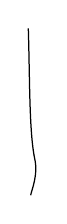
\begin{tikzpicture}[x=1cm,y=1cm]\draw[line width=.45pt] (0,0) .. controls (.02,-.65) and (.01,-1.3) .. (.08,-1.65) .. controls (.13,-1.86) and (.04,-2.06) .. (.03,-2.12);\end{tikzpicture}}

We write $F=F_0\amalg G$, and we apply \unsure{lemma|Lemma}

\deleted{\uline{Corollary 2} Let $(F_i)_{\unsure{j|i}\in I}$ be a family of pairwise disjoint connected components. Then} \deleted{$F=\coprod F_i$} \deleted{the figure generated by the $F_i$ is their disjoint sum $\coprod F_i$} \deleted{and} \deleted{$\subset F$, and if the family is finite (for example $F$} \deleted{finite} \deleted{finite figure) then $F=(\coprod F_i)\amalg H$.}

\deleted{It is not obvious that every nonempty figure has a connected component,} \deleted{the difficulty being in the \unsure{existence} \unsure{or}} \deleted{\unsure{to} subfigures \unsure{``compl. dis''|``complementary''|``contained''}} \deleted{\inserted{But it is true for figures of finite type, and a fortiori for finite figures. The}}

\uline{Proposition} Let $F$ be a figure, $A=\overline F\inserted{\subset M}$ the set of its strata. \deleted{Then the map} For a subfigure \deleted{$F$} $F_0$ of $F$ to be a connected component of $F$, it is necessary and sufficient that $\overline{F_0}$ be a connected component of the ordered set $A$ (for the order induced by $\leq$). We thus find a one-to-one correspondence between the set of connected components
